% SPDX-License-Identifier: Apache-2.0
%
% The conformance report: the RISC-V architectural tests on the Vreteno
% core. Every number comes from results.tex and the tables beside it,
% which //tools/report writes from the runs of the build that typesets
% this file.
\documentclass[journal,9pt]{IEEEtran}

\newcommand{\listingsize}{\fontsize{6}{7}\selectfont}
% SPDX-License-Identifier: Apache-2.0
%
% The house preamble, copied from TxHDL's docs/housestyle.tex so that
% this report is set as the TxHDL documents are. Loaded after
% \documentclass, before \title.
% Computer Modern. IEEEtran selects Times (ptm) by default, so the face has
% to be chosen explicitly.
%
% Latin Modern is the Computer Modern variety used here, and the choice is
% forced rather than aesthetic. Under T1 encoding, plain `cmr` has no Type 1
% outlines unless cm-super is installed, and it is not in the pinned
% distribution, so pdflatex falls back to EC bitmaps and every glyph in the
% PDF becomes a Type 3 font. That was measured: the first build produced a
% document with 10 Type 3 fonts and no Type 1. Latin Modern is Computer
% Modern redrawn with a full T1 repertoire and real .pfb outlines, so the
% same design comes out scalable.
\usepackage[T1]{fontenc}
\usepackage[utf8]{inputenc}
\usepackage{lmodern}
% microtype is not in the pinned TeX distribution. emergencystretch alone
% keeps the two-column measure from producing overfull lines.
\setlength{\emergencystretch}{3em}

\usepackage{amsmath}
\usepackage{amssymb}
\usepackage{amsthm}
\usepackage{booktabs}
\usepackage{array}
% enumitem is not in the pinned TeX distribution; the list spacing below
% does what \setlist would have done.
\usepackage{float}
\usepackage{xcolor}
\usepackage{listings}
\usepackage{tikz}
\usetikzlibrary{arrows.meta,positioning,fit,backgrounds,calc}
\usepackage[hidelinks,bookmarks=true]{hyperref}

% Numbered, definition-style box for a rule the reader is meant to apply.
\theoremstyle{definition}
\newtheorem{rulebox}{Rule}
\newtheorem{example}{Example}

% Unnumbered asides.
\theoremstyle{remark}
\newtheorem*{tip}{Tip}
\newtheorem*{pitfall}{Pitfall}

% Tighter lists, in place of enumitem's \setlist.
\setlength{\topsep}{2pt}
\setlength{\itemsep}{1pt}
\setlength{\parsep}{0pt}

% Code in the running text. The typewriter face under T1 ligates `<<`
% and `>>` into guillemets, so a shift printed as \code{<<} came out as
% a French quotation mark (issue 571). microtype's \DisableLigatures is
% not in the pinned distribution, but the primitive it rests on is
% pdfTeX's own: \pdfnoligatures strips every ligature from the font it
% is given, and the current font inside \texttt is the typewriter face
% at the size in use, so each size is stripped the first time \code
% sets it. Code wants no ligature at all: two quotes are two quotes.
\newcommand{\code}[1]{\texttt{\ifdefined\pdfnoligatures\pdfnoligatures\font\fi #1}}
\newcommand{\term}[1]{\emph{#1}}

% Syntax highlighting. Four roles, distinguishable in colour and still
% distinguishable in greyscale, because an IEEE article gets printed: the
% keyword is the only bold role, the comment is the only italic one, and the
% two remaining roles differ in lightness as well as in hue.
\definecolor{kwblue}{RGB}{20,60,150}
\definecolor{cmtgreen}{RGB}{90,120,90}
\definecolor{strred}{RGB}{150,50,40}
\definecolor{numgray}{gray}{0.45}
\definecolor{framegray}{gray}{0.70}
\definecolor{bgshade}{gray}{0.97}
% A darker fill for figure cells. The listing background has to stay very
% light to keep code readable; a figure cell has to be clearly shaded or the
% distinction it draws is invisible in print.
\definecolor{cellshade}{gray}{0.90}

% The listing size is the document's choice, because it depends on the
% column: a two-column article sets `\listingsize` to 6pt and keeps its
% listings within 70 columns, or to 5.6pt when it includes source that
% rustfmt sets at 80, which is what fits a column's frame (issue 1061);
% a one-column document keeps the body size and includes source files
% at 80. `//docs:frame_test` checks every listing line against its frame. Lines are never broken; a line that does not fit
% overflows the frame, which is visible, rather than wrapping, which is
% not.
\providecommand{\listingsize}{\scriptsize}

% `'` is deliberately not a string delimiter: the language uses it for loop
% labels, as Rust does, so treating it as a quote would swallow the rest of
% the line.
\lstdefinestyle{txhdl}{
  basicstyle=\ttfamily\listingsize,
  keywordstyle=\bfseries\color{kwblue},
  commentstyle=\itshape\color{cmtgreen},
  stringstyle=\color{strred},
  numberstyle=\tiny\color{numgray},
  morekeywords={mod,use,pub,const,type,struct,enum,trait,impl,fn,async,let,mut,
    match,if,else,loop,while,for,in,break,continue,return,as,await,
    module,bus,channel,transaction,protocol,pipeline,flow,seq,config,
    port,stage,pipe,instance,connect,bind,tag,domain,blackbox,foreign,
    property,role,signal,handler,true,false,
    sequence,interface,modport,implements,package,import,var,wire,func,proc,
    case,default,next,fork,branch,join,state,fsm},
  morecomment=[l]{//},
  morestring=[b]",
  showstringspaces=false,
  columns=fullflexible,
  keepspaces=true,
  breaklines=false,
  % Framed, so a listing is bounded rather than floating in the column.
  frame=single,
  rulecolor=\color{framegray},
  framesep=3pt,
  backgroundcolor=\color{bgshade},
  xleftmargin=3pt,
  xrightmargin=3pt,
  aboveskip=6pt,
  belowskip=6pt,
  % Every listing is numbered and captioned, so it can be referred to by
  % number. `caption` without `float` numbers the listing and leaves it
  % where it was written, which is what a listing in running prose needs.
  captionpos=b,
  abovecaptionskip=2pt,
  belowcaptionskip=6pt,
}

% Figures drawn as text. Framed the same way, and with the highlighting
% switched off, because a box-and-arrow diagram is not code and half its
% words turning blue reads as an accident. Setting a style adds keys rather
% than clearing the ones already set, so the three roles are neutralised by
% hand rather than by leaving them out. Program output is printed in this
% style too, and a netlist's assignment can run past the frame, so a line
% that does not fit is broken and the rest indented; source never is.
\lstdefinestyle{ascii}{
  basicstyle=\ttfamily\listingsize,
  keywordstyle=\ttfamily,
  commentstyle=\ttfamily,
  stringstyle=\ttfamily,
  columns=fullflexible,
  keepspaces=true,
  breaklines=true,
  breakindent=2em,
  frame=single,
  rulecolor=\color{framegray},
  framesep=3pt,
  backgroundcolor=\color{bgshade},
  xleftmargin=3pt,
  xrightmargin=3pt,
  aboveskip=6pt,
  belowskip=6pt,
}
\lstset{style=txhdl}

% House TikZ styles. `shorten` lives on the arrow styles rather than on each
% arrow, so every arrow in the document gets the gap, including ones added
% later. TikZ clips a path at a node's border, so without it an arrowhead
% butts against the box with no gap at all. Keep `node distance` well above
% twice the shorten, or the arrow shrinks to nothing.
\tikzset{
  box/.style={draw,rounded corners=2pt,align=center,inner sep=4pt,
              font=\footnotesize},
  boxf/.style={box,fill=bgshade},
  lbl/.style={font=\scriptsize\itshape,align=center},
  fl/.style={-{Stealth[length=4pt]},shorten >=2.5pt,shorten <=2.5pt},
  fld/.style={fl,dashed},
}


% The contents list: the class gives a section's number 2.75em, which
% a Roman numeral past thirty overruns onto the title, so the box is
% wider here, and a subsection's entry starts where a title does.
\makeatletter
\def\l@section#1#2{\addpenalty{\@secpenalty}\addvspace{1.0em plus 1pt}%
    \@tempdima 5.75em \begingroup \parindent \z@ \rightskip \@pnumwidth%
    \parfillskip-\@pnumwidth {\bfseries\leavevmode #1}\hfil\hbox to\@pnumwidth{\hss #2}\par%
    \endgroup}
\def\l@subsection{\@dottedtocline{2}{5.75em}{5em}}
\def\l@subsubsection{\@dottedtocline{3}{10.75em}{5.5em}}
\makeatother


\InputIfFileExists{buildstamp.tex}{}{}
\providecommand{\buildstamp}{Draft build (outside the Bazel flow).}
\input{results}

% Console output of a test, as printed: no highlighting, lines broken.
\lstdefinestyle{console}{style=ascii}
\definecolor{barfill}{RGB}{59,91,146}
\definecolor{tint}{RGB}{232,238,250}
\tikzset{
  art/.style={box,fill=tint},
  tool/.style={box,fill=bgshade},
  chk/.style={box,fill=green!12},
}

\title{RISC-V Architectural Conformance\\of the Vreteno Core}

\author{Filip Filmar%
\thanks{The author is independent, at f@hdlfactory.com.}%
\thanks{This report is generated. A build of the repository
\code{filmil/vreteno-conformance} runs the tests and typesets the
report from the results of that run, every day. Every count, table and
chart in it comes from that build.}%
\thanks{The author used a large language model, Claude, as an assistant
in building the test harness and in writing this report; every commit
of the repository says so and lists the prompts that led to it,
verbatim.}%
\thanks{\buildstamp}}

\markboth{Vreteno conformance, \ReportDate}{Filmar: RISC-V Architectural Conformance of the Vreteno Core}

\begin{document}
\maketitle

\begin{abstract}
Vreteno is a three-stage RV32IMAC core with machine, supervisor and
user modes and Sv32 paging, written in the hardware description
language TxHDL. This report runs the official RISC-V architectural
tests on it. The tests come from RISC-V International's ACT4 suite, and
the Sail reference model computes the result each test must reproduce.
Each test runs on the core's Verilog netlist under Verilator. Of the
\NCatalog{} tests in the catalog, \NTests{} apply to Vreteno, in
\NSuites{} suites. \NRtlPass{} of them pass on the netlist, and
\NSailPass{} pass their own self-check on Sail. Together the tests
compare \NChecks{} values with Sail's. The first run, on 2026-10-07,
had one failure, and it is a real defect: the core cannot set
\code{mstatus.TVM}. A second finding of that run is that the core has
no \code{menvcfg}, so it conforms to version 1.11 of the privileged
specification rather than 1.12. Both are filed as issues against
TxHDL. The build that produces this report fetches
every tool by checksum, and it runs every day against the latest
commit of the core.
\end{abstract}

\begin{IEEEkeywords}
RISC-V, architectural tests, conformance, Sail, Verilator, hardware
verification, TxHDL.
\end{IEEEkeywords}

{\footnotesize\tableofcontents}

% SPDX-License-Identifier: Apache-2.0
\section{Introduction}
\label{sec:intro}

\IEEEPARstart{A}{} processor conforms to RISC-V when every
instruction it implements gives the result the specification defines.
RISC-V International publishes a suite of tests for this, the
architectural tests~\cite{act}. Each test runs a fixed program and
checks the values it computes against values the Sail reference
model~\cite{sail} computed for the same program. A core that passes a
test agrees with the reference model on everything that test checks.

Vreteno is the RISC-V core of the TxHDL project~\cite{txhdl}. It
implements RV32IMAC: the base integer set, multiply and divide, the
atomic instructions and the compressed ones. It also has machine,
supervisor and user modes, Sv32 virtual memory, and an instruction
cache. TxHDL writes the core as a Rust program and lowers it to
Verilog. The project checks that netlist against its own reference
model in lockstep, and it runs on an Artix-7 board.

Those checks say that the core does what its authors meant. The
architectural tests say something else: that what the authors meant is
what the specification says. This report applies them.

The result is short. Of the \NCatalog{} tests in the catalog,
\NTests{} apply to Vreteno, and \NRtlPass{} pass on its netlist, which
is \PassPercent{}\,\%. The tests compare \NChecks{} values with Sail's.
The first run found one real defect in the core, described in
Section~\ref{sec:findings}, and it is the run's one failure.

\subsection{How to read this report}

Section~\ref{sec:tests} says how the tests work.
Section~\ref{sec:dut} describes the device under test: the netlist, the
memory around it, and how a run ends.
Section~\ref{sec:config} says how Vreteno is described to the tests,
and why each choice was made.
Section~\ref{sec:build} describes the build that runs it all.
Sections~\ref{sec:results} and~\ref{sec:findings} give the results and
the defects found.
Section~\ref{sec:limits} lists what this run does not check.
The appendices give the console output of each failing test and a line
for every test.

% SPDX-License-Identifier: Apache-2.0
\section{The architectural tests}
\label{sec:tests}

The architectural tests are assembly programs, one file each, grouped
into suites by extension. This report uses ACT4, the current framework
of the suite, at commit \code{\ActCommit}~\cite{act,ctp}. Each test file
starts with a header that states what the test needs: the extensions it
requires, its \code{-march} string, and any parameter of the core it
depends on, such as XLEN or the number of physical memory protection
entries.

\subsection{Self-checking tests}

An ACT4 test checks itself. It is built twice, and the reference model
runs in between. Fig.~\ref{fig:flow} shows the four steps.

\begin{enumerate}
\item The test is compiled with \code{-DSIGNATURE}. Built this way, it
stores every result it computes into a region of memory called the
signature.
\item Sail runs that program and writes the signature region to a file.
\item The signature is turned into assembler source, one \code{.word}
directive per value.
\item The test is compiled again with \code{-DRVTEST\_SELFCHECK},
including that source. Now each time the test computes a value, it
compares it with Sail's value at the same place, and branches to a
failure routine on a mismatch.
\end{enumerate}

The final program decides for itself whether it passed. It prints
\code{TEST PASSED} or \code{TEST FAILED} on a console, and on a failure
it also prints the instruction, the register, the expected value and
the value it got. A device under test only has to run the program,
provide the console, and report how the program ended.

\begin{figure}[t]
\centering
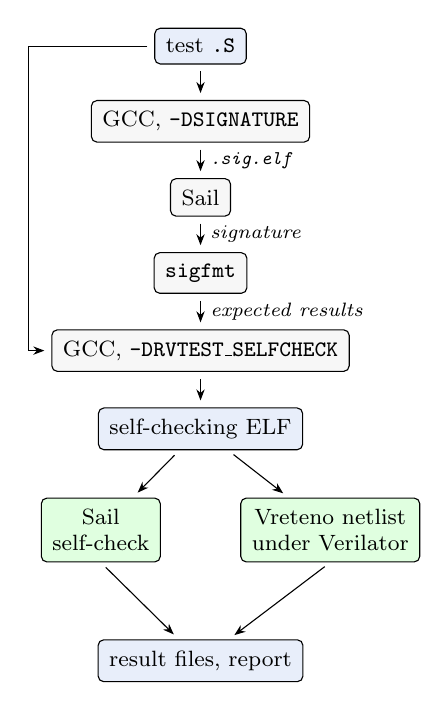
\begin{tikzpicture}[node distance=4.5mm and 3mm, font=\footnotesize]
\node[art] (src) {test \code{.S}};
\node[tool, below=of src] (cc1) {GCC, \code{-DSIGNATURE}};
\node[tool, below=of cc1] (sail1) {Sail};
\node[tool, below=of sail1] (fmt) {\code{sigfmt}};
\node[tool, below=of fmt] (cc2) {GCC, \code{-DRVTEST\_SELFCHECK}};
\node[art, below=of cc2] (elf) {self-checking ELF};
\node[chk, below left=6mm and -8mm of elf] (sail2) {Sail\\self-check};
\node[chk, below right=6mm and -8mm of elf] (rtl) {Vreteno netlist\\under Verilator};
\node[art, below=24mm of elf] (rep) {result files, report};
\draw[fl] (src) -- (cc1);
\draw[fl] (cc1) -- node[lbl,right] {\code{.sig.elf}} (sail1);
\draw[fl] (sail1) -- node[lbl,right] {signature} (fmt);
\draw[fl] (fmt) -- node[lbl,right] {expected results} (cc2);
\draw[fl] (src.west) -- ++(-16mm,0) |- (cc2.west);
\draw[fl] (cc2) -- (elf);
\draw[fl] (elf) -- (sail2);
\draw[fl] (elf) -- (rtl);
\draw[fl] (sail2.south) -- (rep);
\draw[fl] (rtl.south) -- (rep);
\end{tikzpicture}
\caption{How one test becomes two results. Every box is a Bazel action.}
\label{fig:flow}
\end{figure}

\subsection{Which tests apply}

A test applies to a core when the core implements every extension the
test requires and has every parameter value the test states. The
ACT4 framework makes this selection in Python, from a description of
the core in the RISC-V Unified Database format. This build makes the
same selection in Bazel's own language, from a list of extensions and
parameters (Section~\ref{sec:config}). It applies the same rules,
including comparisons such as \code{NUM\_PMP\_ENTRIES: '>0'}.

The selection is made over \NCatalog{} tests: the RV32 suites and the
privileged suites of the catalog. It keeps \NTests{} of them.

% SPDX-License-Identifier: Apache-2.0
\section{The device under test}
\label{sec:dut}

The device under test is Vreteno's netlist, the Verilog that TxHDL
writes for the core. It is the same netlist that the board's
bitstream is built from, so the tests check what is synthesized rather
than a model of it.

\subsection{The wrapper}

The core on its own speaks TxHDL's transaction channels, not a standard
bus. A small TxHDL unit, \code{Dut}, joins three existing parts so that
the netlist has one standard AXI4 manager port (Fig.~\ref{fig:dut}).
The three parts are the hart, which is the core with its memory
management unit; the tracker, which turns the core's loads, stores and
fetches into AXI4 bursts; and an adapter that puts the five AXI4
channels on pins. All three come from TxHDL unchanged. The wrapper is
about 250 lines of Rust, most of them port names, and TxHDL lowers it
with the core into one Verilog file.

\begin{figure}[t]
\centering
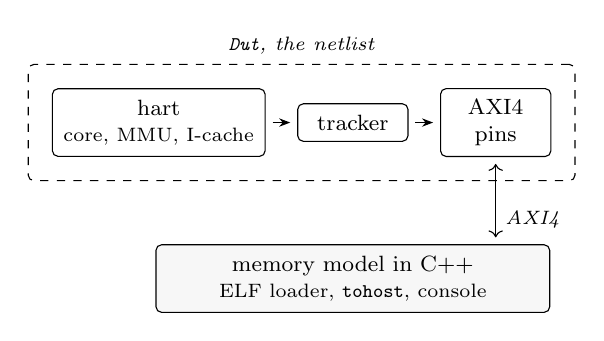
\begin{tikzpicture}[node distance=5mm and 4mm, font=\footnotesize]
\node[box, minimum width=22mm] (hart) {hart\\\scriptsize core, MMU, I-cache};
\node[box, right=of hart, minimum width=14mm] (trk) {tracker};
\node[box, right=of trk, minimum width=14mm] (pins) {AXI4\\pins};
\node[draw, dashed, rounded corners=2pt, inner sep=3mm,
      fit=(hart)(trk)(pins), label={[lbl]above:\code{Dut}, the netlist}] (dut) {};
\node[tool, below=13mm of trk, minimum width=50mm] (mem)
  {memory model in C++\\\scriptsize ELF loader, \code{tohost}, console};
\draw[fl] (hart) -- (trk);
\draw[fl] (trk) -- (pins);
\draw[fl, <->] (pins.south) -- node[lbl, right, pos=0.72] {AXI4} (pins.south |- mem.north);
\end{tikzpicture}
\caption{The device under test. Only the memory model is written for
this testbench; everything inside the dashed box is TxHDL's.}
\label{fig:dut}
\end{figure}

\subsection{Booting into the test}

Vreteno fetches its first 4\,KiB from a memory inside the core, which
the netlist initializes. The wrapper puts two instructions there:
\code{lui t0,0x40000} and \code{jr t0}. They jump to
\code{0x4000\_0000}, where every test is linked. On the board, that
address is the start of DDR3, and the core's instruction cache holds
words from that range. So the tests run from cached memory, as the
board's programs do.

\subsection{The memory and the end of a run}

The testbench is a C++ program around the Verilated netlist. It loads
the test's ELF into a sparse memory and answers every AXI4 burst from
it, with every \code{ready} held high. The interrupt lines and the
debug module's lines are held low.

A test ends the way it ends on Sail, through the HTIF \code{tohost}
word. The testbench reads the word's address from the ELF's symbol
table. A write to its upper half completes a command. Device~1 with
command~1 prints a character on the console. Any other command with an
odd lower half ends the run: 1 means the test passed, and 3 means it
failed.

The testbench writes a result file for each run: the status, the
cycles, the instructions retired, and the console text. A run that
reaches 20 million cycles stops with the status \code{TIMEOUT}. The
build does not stop when a test fails. The result file records the
failure, a test target reads it, and this report counts it.

% SPDX-License-Identifier: Apache-2.0
\section{Describing Vreteno to the tests}
\label{sec:config}

The tests need to know what the core implements. Three files tell
them, and a fourth tells the reference model. All four describe the
same machine, and they are written from the core's source in TxHDL,
\code{cpu/vreteno/src/isa.rs} and \code{core.rs}.

\begin{itemize}
\item \code{rvtest\_config.h} defines a macro for each extension and
parameter. ACT4 generates this file from a Unified Database
description, with Ruby tools; here it is written by hand.
\item \code{rvmodel\_macros.h} says how the device ends a test and
prints a character. Vreteno's testbench speaks HTIF as Sail does, so
one set of macros serves both.
\item \code{link.ld} places the test at \code{0x4000\_0000}.
\item \code{sail.json} configures Sail to behave as Vreteno does where
the specification lets an implementation choose.
\end{itemize}

\subsection{Extensions and parameters}

The extensions are \Extensions. The parameters are XLEN of 32, no
misaligned loads and stores in hardware, and no physical memory
protection. Table~\ref{tab:config} gives the choices that matter for
the tests and the reason for each.

\begin{table}[t]
\centering
\caption{Choices in the description of Vreteno}
\label{tab:config}
\footnotesize
\begin{tabular}{@{}>{\raggedright\arraybackslash}p{0.36\columnwidth}>{\raggedright\arraybackslash}p{0.58\columnwidth}@{}}
\toprule
Choice & Reason in the core \\
\midrule
Privileged version 1.11 & No \code{menvcfg} or \code{senvcfg}
(Section~\ref{sec:findings}). \\
\code{mtvec}, \code{stvec} direct only & The core clears the two mode
bits on a write. \\
Misaligned access traps & A load or store that is not aligned raises
an address-misaligned exception. \\
Misaligned AMO traps as misaligned & The specification allows this or
an access fault; the core does the former. \\
\code{mtval} nonzero & The core writes the instruction for an illegal
instruction, the pc for a breakpoint, the address for a misaligned or
faulting access. \\
A and D bits: Svade & The page walker never writes; a clear A bit, or
a clear D bit on a store, is a page fault. \\
No PMP, no \code{mcountinhibit} & Neither is implemented. \\
\code{mvendorid} and the rest 0 & All four read as zero. \\
\bottomrule
\end{tabular}
\end{table}

\subsection{What is left out}

One suite is left out by hand. The Svade tests begin by clearing
\code{menvcfgh.ADUE}, a register that exists only from privileged
version 1.12. On a 1.11 core the first instruction of the test traps,
and Sail also fails the test in that configuration. The behaviour
Svade names, a page fault on a clear A or D bit, is still tested by the
Sv suite.

Everything else the selection drops, it drops for a stated reason: the
test needs an extension the core lacks, such as F, D or the bit
manipulation extensions, or it needs a parameter the core does not
have, such as physical memory protection entries or misaligned access
in hardware.

% SPDX-License-Identifier: Apache-2.0
\section{The build}
\label{sec:build}

Bazel runs everything in this report, and it fetches every tool it
uses by checksum or by commit. Nothing is installed on the machine
beyond Bazelisk and Git. Table~\ref{tab:tools} lists the tools.

\begin{table}[t]
\centering
\caption{What the build fetches}
\label{tab:tools}
\footnotesize
\begin{tabular}{@{}lp{0.6\columnwidth}@{}}
\toprule
Tool & Version and source \\
\midrule
Vreteno & TxHDL commit \code{\TxhdlCommit}, from its GitHub mirror \\
Tests & riscv-arch-test commit \code{\ActCommit} \\
Reference & \SailVersion, prebuilt release \\
Compiler & \GccVersion \\
Simulator & Verilator 5.046, TxHDL's prebuilt binary \\
C and C++ & LLVM over a pinned Debian sysroot, from TxHDL \\
\LaTeX & a pinned TinyTeX, with TxHDL's copies of IEEEtran, pgf and
listings \\
\bottomrule
\end{tabular}
\end{table}

\subsection{From test file to target}

A repository rule downloads the test suite and reads the configuration
header of every test file. It writes the headers into a list that the
build reads when it analyses the targets, so that selecting the tests
needs no Python. For each selected test, a Bazel macro makes one
target that builds the self-checking ELF in the four steps of
Fig.~\ref{fig:flow}. It makes two more targets that run the ELF, one on
Sail and one on the netlist, and a test target for each run.
\code{sigfmt}, the tool in step three, is a short Rust program. It
replaces the Python function in ACT4 that does the same job.

Each step is an action with declared inputs and outputs, so Bazel runs
the \NTests{} tests in parallel and caches every step. A change to the
core reruns the netlist runs and nothing else. A change to the
description of the core rebuilds every ELF.

\subsection{Known failures}

A test that the core is known to fail is listed with the URL of the
issue that tracks it. Its test target then passes while the run fails,
and fails once the run passes. The list therefore shrinks when the
core is fixed, and \code{bazel test} stays useful for changes to the
harness while a defect is open. This report reads the result files,
not the test targets, so a known failure counts as a failure here.

\subsection{Every day}

A workflow runs the build every day against the newest commit of
TxHDL. It typesets this report, publishes it as a release of the
repository, and publishes the same results as a web page on
hdlfactory.com. The commit of the core and the date are in the title
footnote of every copy.

% SPDX-License-Identifier: Apache-2.0
\section{Results}
\label{sec:results}

On \ReportDate, \NRtlPass{} of the \NTests{} tests passed on Vreteno's
netlist. The failures, \NRtlFail{} in all, divide into two kinds:
known failures, each tracked by an issue (\NKnownFail), and new ones
(\NUnknownFail).
\NSailPass{} of the \NTests{} tests passed their self-check on Sail. The
Sail column is a check on the harness rather than on the core: each
self-checking program must pass on the model that wrote its expected
values. When it does, the description of the core, the compiler flags
and the test sources agree with one another.

Table~\ref{tab:suites} gives the results by suite. The checks column
counts the values a test compares with Sail's. The counts exclude the
fill of the unused signature area and the marker words. The suite that
compares the most is \code{\MostChecksSuite}, with \MostChecks{}
values in \MostChecksTests{} tests.

\begin{table}[t]
\centering
\caption{Results by suite}
\label{tab:suites}
\scriptsize
\input{suites}
\end{table}

\subsection{Cycles}

The \NTests{} runs took \TotalCycles{} cycles to retire \TotalInstr{}
instructions, \MeanCPI{} cycles per instruction on average.
Fig.~\ref{fig:cpi} breaks this down by suite.

These numbers describe the testbench as much as the core. An
architectural test is long straight-line code that runs once. The
instruction cache then helps only within a line of four words, and
each new line is fetched over the bus. The slowest suite is \code{\SlowSuite}, at \SlowCPI{} cycles
per instruction, and the fastest is \code{\FastSuite}, at \FastCPI.
The multiply and divide instructions take several cycles each in
Vreteno's sequencer, which is why \code{M} and \code{Zmmul} are above
the rest. The figures are a record that the runs completed
at a plausible speed. They are not a performance claim.

\begin{figure}[t]
\centering
\input{cpichart}
\caption{Mean cycles per instruction on the netlist, by suite.}
\label{fig:cpi}
\end{figure}

% SPDX-License-Identifier: Apache-2.0
\section{Findings}
\label{sec:findings}

The first run, on 2026-10-07 against TxHDL commit \code{894cc2e3b296},
found two departures from the specification. Both are filed as issues
against TxHDL, and both are in the privileged architecture. In that
run, every unprivileged instruction the core implements matched Sail
on every value the tests check. A later run that fails anything else
shows it in Section~\ref{sec:results} and in
Appendix~\ref{sec:failures}, as a failure that is not known.

\subsection{\code{mstatus.TVM}, \code{TW} and \code{TSR} cannot be set}

The test \code{SvSm\_sv\_mstatus\_tvm\_test-00} sets \code{mstatus.MPP}
to 3 and \code{mstatus.TVM} to 1, then reads \code{mstatus} back. Sail
reads \code{0x00101800}. Vreteno reads \code{0x00001800}: the TVM bit,
bit 20, did not stick. The test's own console output is in
Appendix~\ref{sec:failures}.

The cause is in the core's write mask for \code{mstatus},
\code{MSTATUS\_W = 0x000e\_19aa}, which leaves out bits 20, 21 and 22:
TVM, TW and TSR. The privileged specification requires all three to be
writable when supervisor mode is implemented~\cite{priv}. Without them,
machine mode cannot trap a supervisor's \code{satp} accesses and
\code{sfence.vma}, nor its \code{wfi} and \code{sret}. A hypervisor or
a monitor that emulates those instructions relies on these traps.
The issue is TxHDL issue 1347~\cite{issue1347}.

\subsection{No \code{menvcfg} and no \code{senvcfg}}

Version 1.12 of the privileged specification adds \code{menvcfg}, which
a core must have when it implements user mode, and \code{senvcfg},
which it must have when it implements supervisor mode. Vreteno has
neither, and an access to either raises an illegal instruction
exception. Described as a 1.12 core, Vreteno fails every test: the
tests write \code{menvcfg} while they boot. Described as a 1.11 core,
it passes all but one.

The core does have \code{mstatush}, which is also new in 1.12, so it
sits between the two versions. This report describes it as 1.11, and
the Svade suite, which needs \code{menvcfgh}, does not run. The issue
is TxHDL issue 1348~\cite{issue1348}. Adding the two registers, with
their fields read-only zero where the core lacks the feature, would
let the core be described as 1.12 and the Svade suite run.

\subsection{Since the first run}

TxHDL fixed both issues by commit \code{48daf9778add}, and the run of
2026-10-08 against that commit passes
\code{SvSm\_sv\_mstatus\_tvm\_test-00}. The core now has
\code{menvcfg} and \code{senvcfg} too, but this report still
describes it as a 1.11 core, so the Svade suite still does not run.

The same commit adds a data cache for the DDR3, and with it five tests
fail that passed before: the byte, halfword and word loads,
\code{I-lb-00}, \code{I-lbu-00}, \code{I-lh-00}, \code{I-lhu-00} and
\code{I-lw-00}. Each fails where it stores a new value to a line the
cache holds and loads it back at once. The load returns the value the
case before it stored. The tests run in the cached range of the
address space, and the uncached path has no such failure. The issue is
TxHDL issue 1431~\cite{issue1431}. TxHDL fixed it by commit
\code{e9681300a8b2}, and the run of 2026-10-09 against that commit
passes all five tests.

\subsection{A choice that is not a defect}

The first run had six more failures, all in tests of atomic
instructions at misaligned addresses. Vreteno raised
address-misaligned there, and the first configuration of Sail expected
an access fault. The specification allows either. The fix was in
\code{sail.json}, which now says that the core raises address-misaligned,
and the six tests pass.

% SPDX-License-Identifier: Apache-2.0
\section{What this run does not check}
\label{sec:limits}

A passing run says that Vreteno agrees with Sail on the values the
selected tests check. It does not say more than that, and five gaps
are worth stating.

\begin{itemize}
\item \textbf{Interrupts.} The testbench raises no interrupt, so the
tests that need a timer or an interrupt controller are not selected.
The core's interrupt path is checked by TxHDL's own tests, not here.
\item \textbf{The Svade suite} does not run, for the reason in
Section~\ref{sec:findings}.
\item \textbf{One simulator.} The netlist runs under Verilator only.
TxHDL also writes VHDL, and its own tests run that under nvc, but the
architectural tests do not.
\item \textbf{The description is written by hand.} If
\code{rvtest\_config.h} or \code{sail.json} claims a behaviour the core
does not have, the tests check the claim. A self-check on Sail
catches a description that disagrees with itself, not one that
disagrees with the core. The table of choices in
Section~\ref{sec:config} is what a reviewer should check against the
core's source.
\item \textbf{The board.} The tests run on the netlist in simulation,
with a memory model, not on the Artix-7 board with its DDR3.
\end{itemize}

% SPDX-License-Identifier: Apache-2.0
\section{Conclusion}
\label{sec:conclusion}

The official RISC-V architectural tests now run on Vreteno's netlist,
every day, with every tool fetched by the build. In this run,
\NRtlPass{} of the \NTests{} tests that apply to the core pass. The
first run found a real defect: \code{mstatus.TVM}, \code{TW} and \code{TSR}
cannot be set. The run also found that the core lacks the environment
configuration registers of privileged version 1.12.

Both were filed, and TxHDL fixed both the next day. The run that day
showed the loop working: the TVM test started to pass, its entry in
the list of known failures had to go, and the same run caught a new
defect in the core's data cache within hours of its commit. That
defect was fixed the day after, and the five tests it broke pass
again.


\appendices
\section{The failing tests}
\label{sec:failures}
\input{failures}

\section{Every test}
\label{sec:every}
Tables~\ref{tab:tests} and after list each test with the values it
checks, the cycles its run took on the netlist, and its cycles per
instruction. A test's name is shown without the name of its suite.
\input{tests}

\begin{thebibliography}{10}
\bibitem{act}
RISC-V International, ``RISC-V Architectural Certification Tests,''
\url{https://github.com/riscv-non-isa/riscv-arch-test}, commit
\code{\ActCommit}.

\bibitem{ctp}
RISC-V International, ``Certification Test Plan,''
\url{https://riscv.github.io/riscv-arch-test/ctp.html}.

\bibitem{sail}
RISC-V International, ``Sail RISC-V model,''
\url{https://github.com/riscv/sail-riscv}, release 0.15.

\bibitem{priv}
RISC-V International, \emph{The RISC-V Instruction Set Manual, Volume
II: Privileged Architecture}, versions 1.11 and 1.12.

\bibitem{txhdl}
F.~Filmar and D.~Jankovi\'c, ``TxHDL: A Hardware Description Language
That Is a Rust Library,'' \url{https://www.hdlfactory.com/txhdl/},
2026.

\bibitem{verilator}
W.~Snyder et al., ``Verilator,'' \url{https://verilator.org}.

\bibitem{issue1347}
TxHDL issue 1347, ``mstatus.TVM, TW and TSR are not writable,''
\url{https://git.hdlfactory.com/HDL/txhdl/issues/1347}.

\bibitem{issue1348}
TxHDL issue 1348, ``no menvcfg or senvcfg, so the core is privileged
version 1.11,''
\url{https://git.hdlfactory.com/HDL/txhdl/issues/1348}.
\end{thebibliography}

\end{document}
